%!TEX root = ../report.tex

%
% Architecture
%

\section{Proposed Solution}

We now describe our proposed solution. Since our goal is to have a
highly scalable system with reliability and persistence in mind, we
decided to take advantage of the IPFS ecosystem and all of its different
modules. Our pub-sub module will provide an alternative to the naive
implementation of pub-sub, currently in place in IPFS. The modularity of
the IPFS system allows users to choose what is more convenient for them.
Besides, the existence of a base implementation allows us to have a
baseline for improvement, one from which we can extract metrics and
relevant data.

We will start by covering our subscription model and the multiple
structures that describe events and subscriptions. Afterwards we will
take a closer look at the overlay structure used. We will then cover how
the system works in terms of subscription management, focusing on how
new subscriptions are handled, how new topics are issued and how the
topic hierarchy works. Finally we will cover event dissemination
followed by quality of service, focusing on the mechanisms we have used
to bring persistence, fault tolerance and delivery guarantees to the
network.

\subsection{Subscription Model and Data
Structures}\label{subscription-model-and-data-structures}

Our subscription model follows a topic based approach. It has however
some nice properties that make it far more expressive than what would be
expected of a regular topic based system. To do this, we take advantage
of the core structure of IPFS, the Merkle DAG, through its previously
described interface IPLD. We start by defining two basic structures: the
\emph{topic descriptor} and the \emph{event descriptor}.

The \textbf{topic descriptor} defines the basic structure of our topics.
It is \emph{versioned} by default and possesses links (or merkle-links
as it is referred to in the IPLD specification) to its sub-topics. A
\emph{metadata} object also helps to store other relevant information
such as the protocol version. The following is an example using the JSON
format which IPLD uses.

\begin{verbatim}
{
  name: <topic-name>,
  metadata: <json-object>, // creation date, protocol version, etc.
  #: {
    <sub-topic-name>: <merkle-link to topic descriptor>,
    ...
  },
  parent: <merkle-link to topic descriptor>
}
\end{verbatim}

These structures are addressed by the hash of its content, which in IPFS
are referred to as Content Identifiers~\footnote{https://github.com/ipld/cid} or CID. In
fact, given the definition of these objects, all the content of the
structure itself is addressable based on its CID. For example, if we had
a topic descriptor with a CID
\emph{<foobar-hash>u} we could
address it using a UNIX path approach such as
\emph{/<foobar-hash>}. However we
could access its properties directly such as
\emph{/<foobar-hash>/\#} to get the
sub-topics list, or
\emph{/<foobar-hash>/parent} to get
the previous version of this topic. These paths are referred to under
IPFS as \emph{merkle-paths}.

Given the immutable nature of the IPLD structure, the parent link allows
us to create new updated versions of the topic descriptor (with a new
sub-topic for example) while maintaining a history of previous topic
descriptors for this topic. The key \emph{\#} on the other hand
contains a JSON object with merkle-links for all of sub-topics indexed
by name.

The topic name is a string following a UNIX like path pattern. For
example \emph{/sports}. If we are speaking about sub-topics though,
there is an extra requirement, given that a sub-topic name needs to be
consistent with its parent hierarchy. This means that, for a topic
\emph{/sports}, it cannot have a sub-topic \emph{/fruits}, or
\emph{/fruits/apples}. \emph{/sports/football} however is a valid
example.

The \textbf{event descriptor} defines the structure of our events. Each
object has links to its \emph{topic} and its \emph{parent} which
represents the previous event in this stream. A \emph{metadata} object
is used to store creation timestamps an other relevant information. The
\emph{publisher} key will be a reference to the ID of the publisher
node. Finally we have the \emph{payload} object, which will contain the
actual information of the event. The following is an example of it.

\begin{verbatim}
{
  topic: {
    name: <topic-name>, // Name of the topic
    link: <merkle-link> // Link to the topic of this message
  },
  publisher: <publisher node ID>
  parent: <merkle-link to previous event>,
  metadata: <json-object>, // Timestamp and other relevant info
  payload: <json-object>, // The actual message content
}
\end{verbatim}

It is worth noticing the importance of both \emph{parent} links in each
structure. These allow both graph structures to build a complex history.
On one side we have the topic descriptors with a versioning system and
on the other we have a stream of events represented as a chain of
immutable objects. These concepts are very important for the overall
system.

We still need however one more structure to help us build our system.
Given the immutability of the objects above, we need a way to point to
the latest version of a given topic descriptor so that other peers can
easily find it. Fortunately, this scenario is already covered by the
IPFS ecosystem through IPNS~\footnote{https://github.com/ipfs/specs/tree/master/iprs}, which aims at
providing mutability over all these immutable structures. An IPNS record
has a special CID, generated through the hash of a public key from a
cryptographic key pair. These records can be used to point to a specific
CID and are generated using asymmetric cryptography to sign the record.
The records are ephemeral though, so it requires the owner of the
asymmetric keys to republish the record every 24 hours. We have two
important guarantees with this structure: mutability, which allow
creators of topics to point to a new version of a topic descriptor
seamlessly, keeping the same CID as an entry point for the topic;
authenticity of the given topic, given that peers can check the IPNS
record signature and decide if they trust the peer owning that record or
not.

\begin{figure}[hb!]
  \centering
  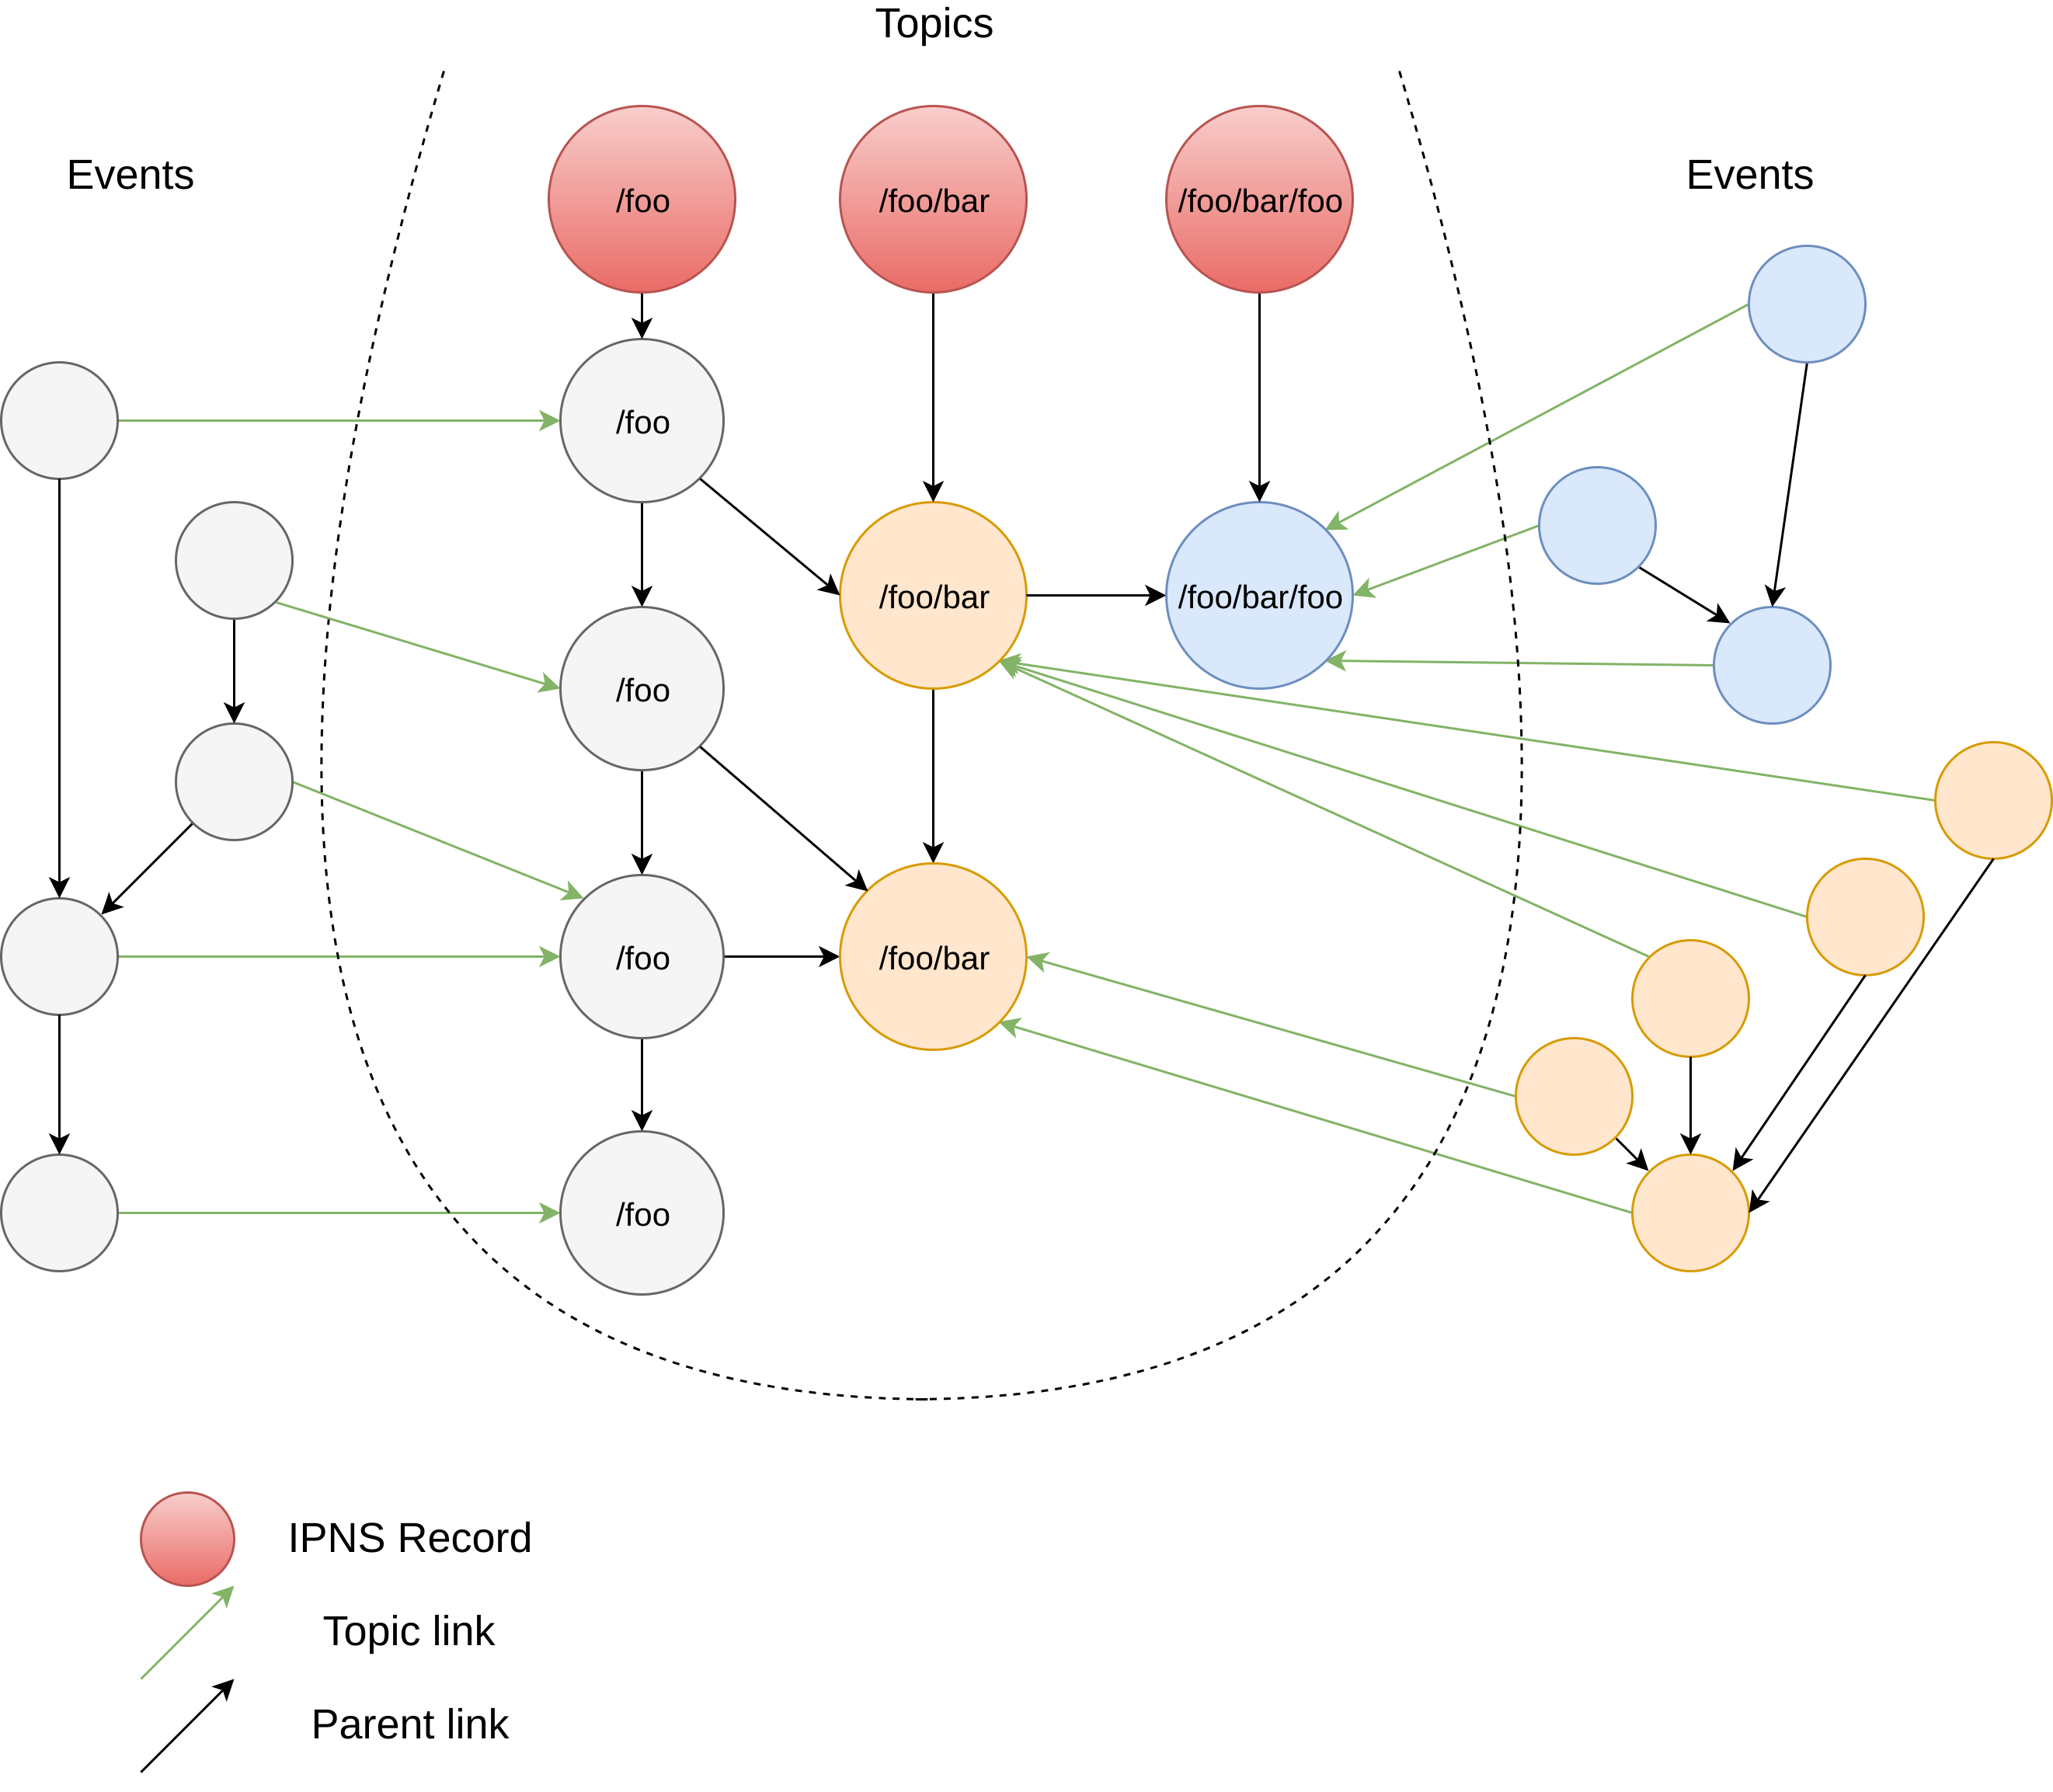
\includegraphics[width=0.95\textwidth]{img/solution-arch.png}
  \caption{caption}
  \label{fig:solution-arch}
\end{figure}

\subsection{Overlay Structure}\label{overlay-structure-solution}

Since our work will be a libp2p compatible module, we will be able to
leverage the multiple modules that already exist in libp2p ecosystem.
This includes network transports, discovery and routing mechanisms as
well as other useful data types and utility methods. The figure \ref{fig:libp2p-stack}
illustrates where our work will take place and
some of the other modules we will be able to use. In order to understand
it though there are some key aspects around libp2p that we need to cover
first. libp2p tries to separate concerns of peer communication and data
transports. In order to do that, it has different transport implementations
under a common interface~\footnote{https://github.com/libp2p/interface-transport},
which can then be leveraged through lip2p-swarm~\footnote{https://github.com/libp2p/js-libp2p-swarm},
a connection abstraction that can deal with multiple
connections under different protocols. On top of this we then have the
peer communication, which can be split into two big mechanisms. On one
end we have the discovery mechanisms~\footnote{https://github.com/libp2p/interface-peer-discovery},
which focus on ways of finding and connecting to new peers.
On the other end we have peer routing~\footnote{https://github.com/libp2p/interface-peer-routing},
which focus on transferring data between already connected
peers. Our work will mostly reside in three different modules: the
pub-sub module implementation; adding extra functionality to the
Kademlia DHT peer routing module; building a small module to power
gossip based communication between peers.

\begin{figure}[hb!]
  \centering
  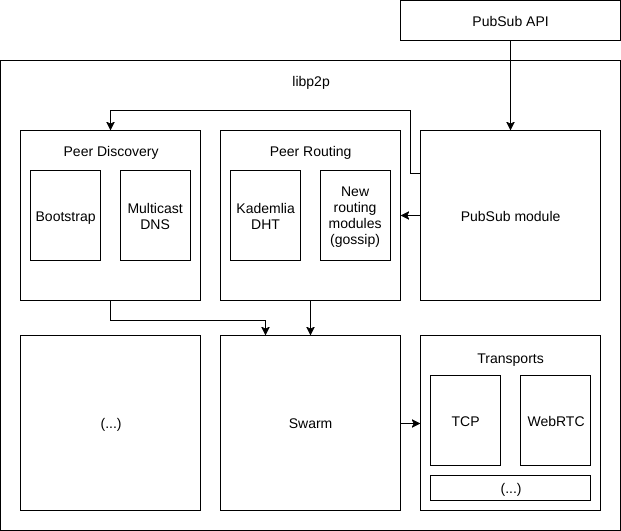
\includegraphics[width=0.95\textwidth]{img/libp2p-stack.png}
  \caption{caption}
  \label{fig:libp2p-stack}
\end{figure}

IPFS currently relies on a Kademlia DHT implementation to provide a
structured overlay mechanism through which it can route messages. We
plan on using this same overlay as a routing mechanism for our system.
In order to do that we have to understand the methods already provided
by it.

\begin{itemize}
  \item
    \textbf{put}: insert a value with a given key in the DHT.
  \item
    \textbf{get}: get a value of given key from the DHT.
  \item
    \textbf{findPeer}: find the peer with the given peer ID in the DHT.
  \item
    \textbf{findPeerLocal}: find the peer with the given peer ID in the
    list of peers to which we are already connected to.
  \item
    \textbf{getClosestPeers}: find the \emph{k}(system wide parameter)
    closest peers to a given key.
  \item
    \textbf{provide}: let the network know that this peer can also
    distribute a given key.
  \item
    \textbf{findProviders}: find providers for a given key.
\end{itemize}

Some methods are basic functions of Kademlia as explained in the
previous section (e.g. \emph{getClosestPeers} is basically a \emph{node
lookup} operation). However, some of these methods are not part of the
Kademlia definition, specifically \emph{provide} and
\emph{findProviders}. The way the \emph{provide} method works is by
setting special records at the node that is housing the key we want to
provide. This way, when peers query for providers or for the actual
content, the Kademlia routing mechanism will ensure that the message
will arrive at the same set of nodes consistently.

We also make use of a gossip based communication mechanism to build a
simple unstructured overlay. We will cover its use case later but in
functionality terms it is quite simple. At each node a fixed size list
of peers should be kept, with its size being a system wide parameter.
Periodically, the nodes should exchange its lists and update info
accordingly. Finally the module should support a simple network flood,
disseminating info across all the nodes.

\subsection{Subscription Management}\label{subscription-management}

In our system, subscriptions are represented as multicast trees, with a
different tree per topic. When a new subscription is issued, a peer,
having the CID of an IPNS record for a given topic, will issue a
\emph{getClosestPeers} method for that given CID. These peers are in
charge of acting as a \emph{rendezvous} for incoming subscriptions and
events. Similar to Scribe, when performing the recursive node lookup
mechanism, at each step, the initiator peer checks to see if some of the
peers that resulted from this step are already part of the multicast
tree. In an affirmative case, the initiator node joins the tree as a
child of this specific node, if not, it chooses the closest one and
issues a special command for this peer to join the multicast tree. The
node upon receiving a command to join the multicast tree registers the
initiator node as its child on the multicast tree and again repeat the
same process until eventually a node belonging to the tree is found.

Peers that belong to a multicast tree are responsible for making sure
that both parent and children nodes are healthy (through periodic pings)
and reconstructing the tree at their level if needed be. For that, they
keep extra state on extra levels of the tree. However, if a network
partition causes these mechanisms to fail, nodes can always rejoin the
network through the procedure detailed above.

Since our system accounts for topic hierarchy, it is possible to create
sub-topics. If a peer wants to add a sub-topic to a topic he created,
all he needs to do is add a new sub-topic link to the parent topic
descriptor and afterwards issue a new IPNS record pointing to the new
version of the parent topic descriptor. If the node does not own the
parent topic it will need to request for the new sub-topic to be added
to the node responsible for the parent topic. If the request is accepted
the procedure will be the same as the one described previously.

It is important to notice that, in our topic hierarchy, subscribers of a
parent topic will not automatically be subscribed to the sub-topics of
it. It is easy however to subscribe to these, since whenever a new
update to the topic descriptor is made, the node responsible for the
topic will issue a special event and disseminate it through the
multicast tree. Since updates to the sub-topic list will trigger topic
descriptor updates, subscribers only have to monitor for changes on the
special key \emph{\#} of the topic descriptor.

\subsection{Event Dissemination}\label{event-dissemination}

Event dissemination in our system is a matter of propagating the event
through the multicast tree. Nodes that are already part of the tree just
need to send the event through the different links the participant has.
For nodes not part of the tree it is just a matter of targeting the
\emph{rendezvous} nodes. A really important note though is that before
disseminating the event through the multicast tree, the publisher should
always invoke the \emph{put} method of the DHT with the event and
respective CID. This will ensure the persistence of the event and help
with the delivery guarantees which we will later discuss.

\subsection{Quality of Service}\label{quality-of-service}

We will now discuss the mechanisms we employ in order to provide the
quality of service guarantees we set as goals for this system. We will
cover the fault tolerance mechanisms, the delivery guarantees and data
persistence.

Looking at \textbf{fault tolerance} we should start by the
\emph{rendezvous} nodes. We need to make sure these do not become a
bottleneck for the system. Hence the usage of the \emph{k} closest nodes
of the given topic CID, this way, through the existing DHT, we get a
natural mechanism for selecting replicas for the \emph{rendezvous} node.
When a new topic is created, the node responsible for creating it is
also responsible for calculating the \emph{k} closest nodes to the topic
CID and communicating with the peers in order for them to become part of
the network. To keep the \emph{rendezvous} nodes synchronised, a simple
gossip overlay is used (described in the previous sections). Another
approach is to use the \emph{provide} method of the DHT as a mechanism
for a node to register as a \emph{rendezvous}.

We then need to cover the IPNS record issue, for it can also become a
bottleneck. An important thing to keep in mind though is that the IPNS
records comes with a notion of ownership which, if you take a closer
look, actually make sense here. Since the peer that created the topic is
actually responsible for updating the respective descriptor and serving
as \emph{rendezvous} for the network. This ownership however does not
translate at all in lock in though, the usage of these graph structures
allows anyone who wants to, to create a new topic based on any previous
topic that you do not even need to own. Better yet, you get all the
topic history and previous event streams connected to this new graph,
for free. With that said, if a set of peers really wants to create a
mechanism where the failure of the node that created the topic does not
imply that the current IPNS record will eventually disappear, they will
need to share the key pair responsible for the record among them, so
that they can keep renovating it in case of failure. This of course will
imply some kind of consensus between the peers, which is outside of the
scope of this work.

On the \textbf{delivery guarantee} front we developed a simple mechanism
that ensures that every node subscribed to a given topic will eventually
get the same event stream as every other node in the network. This is
because of the way the event stream is linked. Given that through the
\emph{parent} key of an event descriptor, a node can check if it is
missing any message from the stream. If it is, it will query the
Kademlia DHT using the \emph{get} method for that specific key. This
approach can ultimately been seen as a simple \emph{NAK} (a negative
ACK) mechanism.

Finally, on the \textbf{persistence} front, we see these graph
structures as the key to create a P2P pub-sub system that finally
addresses data persistence properly. In order to this, having easily
addressable structures is not enough. As such, we devised a way to
guarantee a smooth mechanism for replicating event data. When
propagating an event through the multicast tree, each peer will, with a
given probability \emph{p} (a system wide parameter) invoke the
\emph{provide} method for this specific event. This ensures data is
persisted across multiple nodes which will allow for peers to eventually
build their event stream from any given point. Hence our last mechanism,
when a peer subscribes to a new topic, it will almost immediately
receive the set of leaf events from the graph stream. This simple
approach will give him the ability to rebuild the stream of events as
far as it likes.
